\section{Electron in EM field}
\subsection{Review of Spin}
We have the spin commutation algebra (identical to the angular momentum commutation algebra):
\begin{equation}
    [S_i, S_j] = i\e_{ijk}S_k.
\end{equation}
However, there is no way to represent the spin operators in spatial coordinate; we instead use matrices. Consider $s = 1/2$. Then we have $\v{S} = \frac{1}{2}\gv{\sigma}$, where $S_z$ has eigenstates $\ket{\uparrow} \cong \binom{1}{0}$ and $\ket{\downarrow} \cong \binom{0}{1}$. Any state can be expressed as a linear combination of these two:
\begin{equation}
    \chi = \frac{c_+}{\sqrt{\abs{c_+}^2 + \abs{c_-}^2}}\m{1\\0} + \frac{c_-}{\sqrt{\abs{c_+}^2 + \abs{c_-}^2}}\m{0\\1}.
\end{equation}

\subsection{Inner and Outer Products, Completeness}
We also have the inner product that gives us numbers:
\begin{equation}
    \braket{\uparrow}{\uparrow} = \m{1 & 0}\m{1\\0} = 1.
\end{equation}
Also note that outer products give us matrices:
\begin{equation}
    P_+ = \dyad{\uparrow}{\uparrow} \cong \m{1\\0}\m{1&0} = \m{1&0\\0&0}
\end{equation}
The above $P_\uparrow$ is a projector (that projects onto the spin-up subspace); as we have:
\begin{equation}
    P_\uparrow\ket{\uparrow} = \uparrow, P_+\ket{\downarrow} = 0.
\end{equation}
Note also the completeness relation:
\begin{equation}
    \dyad{\uparrow}{\uparrow} + \dyad{\downarrow}{\downarrow} = \II.
\end{equation}
As $\set{\ket{\uparrow}, \ket{\downarrow}}$ is an ONB for the spin-1/2 Hilbert space. When we have infinitely many states in an ONB, we have:
\begin{equation}
    \sum_{n=0}^\infty \dyad{n}{n} = \mathbb{I}, \quad \int \dyad{x}{x}dx = \mathbb{I}
\end{equation}
where the former is for a discrete ONB, the latter is for a continuous one (of course there are the caveats that $\ket{x}$ aren't really square-integrable states, but let us not worry about this). Now, a question: what is the $\dyad{\uparrow}{\downarrow}$? It is an operator that flips a down-spin to an up-spin:
\begin{equation}
    \dyad{\uparrow}{\downarrow} \cong \m{0&1\\0&0}
\end{equation}
Of course this is just the $S_+$ operator (it is not Hermitian, while $P_\uparrow$ is).

\subsection{Electron in Magnetic Field}
Consider the Hamiltonian:
\begin{equation}
    H = -\gv{\mu}\cdot \v{B}
\end{equation}
where $\gv{\mu} = \gamma\v{S}$ with $\gamma$ is a scalar known as the gyromagnetic ratio. It is equal to:
\begin{equation}
    \gamma = \frac{e\hbar}{2mc}2
\end{equation}
Note we've written $\gamma$ to include the $\hbar$ factor; usually $\hbar$ goes with $\v{S}$, but with our units convention, we prefer to write it this way. Note that if we calculate the gyromagnetic moment just by classical methods, we would just get $\frac{e}{2mc}$. The coefficient $2$ is the $g$-factor, which can be obtained by taking the nonrelativistic limit of the Dirac equation (we won't try to do this here); there is some hidden deep physics here we will leave for a different course.

Note that we have assumed that there is no orbital angular momentum for the electron (we only consider the intrinsic spin); a full treatment would take:
\begin{equation}
    \gv{\mu} = \frac{e\hbar}{2mc}\left(2\v{S} + \v{L}\right).
\end{equation}

\subsection{Electron in Magnetic Field in a single direction}
Now, we suppose a more specific scenario, where $\v{B}$ is aligned along the $z$-axis. We then have:
\begin{equation}
    H = -\gamma B_z\frac{1}{2}\pauliz.
\end{equation}
We have two easily solved eigenvalue equations:
\begin{equation}
    H\chi_+ = E_+\chi_+, H\chi_- = E_-\chi_-.
\end{equation}
Where $E_+ = -\frac{1}{2}\gamma B_z$ and $E_- = \frac{1}{2}\gamma B_z$. Now, a question; why is there a minus sign in $H$? The convention is such that the dipole moment wants to align with the magnetic field. 

Note that in our problem here, the $+$ denotes that we have a upwards projection (and a negative energy, as it is pointed along the field). Conversely, $-$ denotes that we have a downwards projection (and a positive energy). Of course, we know that:
\begin{equation}
    \chi_+ = \m{1\\0}, \chi_- = \m{0\\1}.
\end{equation}
and now everything is solved! We know the eigenvalues and eigenstates, so we have everything we need to determine the Schrodinger time evolution of the quantum state. We can say that:
\begin{equation}
    \chi(t) = \frac{c_+e^{-i\frac{E_+t}{\hbar}}}{\sqrt{\abs{c_+}^2 + \abs{c_-}^2}}\m{1\\0} + \frac{c_-e^{-i\frac{E_-t}{\hbar}}}{\sqrt{\abs{c_+}^2 + \abs{c_-}^2}}\m{0\\1}
\end{equation}

\subsection{Time-dependence of Observables}
For a most general spin-1/2 state, if we enforce the normalization condition of $\abs{c_+}^2 + \abs{c_-}^2 = 1$, then we can parameterize with just three parameters:
\begin{equation}\label{eq-chigeneral}
    \chi = e^{i\alpha}\m{\cos\frac{\theta}{2} \\ \sin\frac{\theta}{2}e^{-i\phi}}
\end{equation}
For now, let us discard the phases ($\alpha = \phi = 0$) and suppose that at $t = 0$ we have:
\begin{equation}\label{eq-chithetat0}
    \chi(t = 0) = \m{\cos\frac{\theta}{2} \\ \sin\frac{\theta}{2}}.
\end{equation}

Question: Let us compute:
\begin{equation}
    \avg{S_z}(t) = \bra{\chi(t)}S_z\ket{\chi(t)}.
\end{equation}
This turns out to be independent of time; let us see this in two ways. First, we can do the explicit calculation. $\chi(t)$ is given by:
\begin{equation}
    \chi(t) = \m{\cos\frac{\theta}{2} e^{i\omega t/2} \\ \sin\frac{\theta}{2} e^{-i\omega t/2}}
\end{equation}
Where $\omega$ is defined as the difference between the two frequencies. When we do the explicit computation, we find:
\begin{equation}
    \bra{\chi(t)}S_z\ket{\chi(t)} = \m{\cos\frac{\theta}{2} e^{-i\omega t/2}& \sin\frac{\theta}{2} e^{i\omega t/2}}\pauliz \m{\cos\frac{\theta}{2} e^{i\omega t/2} \\ \sin\frac{\theta}{2} e^{-i\omega t/2}} =  \frac{1}{2}\left(\cos^2\frac{\theta}{2} - \sin^2\frac{\theta}{2}\right) = \frac{1}{2}\cos\theta.
\end{equation}
If we do the same comnputation for $\avg{S_x}(t)$, we find that the time-dependence does not cancel out:
\begin{equation}
    \bra{\chi(t)}S_x\ket{\chi(t)} = \m{\cos\frac{\theta}{2} e^{-i\omega t/2}& \sin\frac{\theta}{2} e^{i\omega t/2}}\paulix \m{\cos\frac{\theta}{2} e^{i\omega t/2} \\ \sin\frac{\theta}{2} e^{-i\omega t/2}} =  \frac{1}{2}\sin\frac{\theta}{2}\cos\frac{\theta}{2}\left(e^{i\omega t} + e^{-i\omega t}\right) = \frac{1}{2}\sin\theta\cos(\omega t).
\end{equation}
We can picture this as the spin precessing at a fixed angle $\theta$ (fixed $z$-position).

\begin{figure}[htbp]
    \centering
    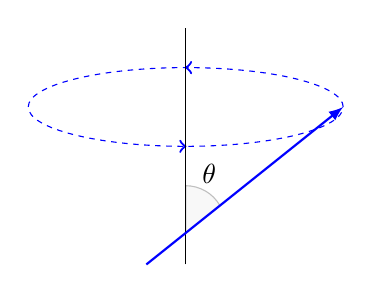
\begin{tikzpicture}
        \draw [rotate around={0.:(0.,0.)},dash pattern=on 2pt off 2pt, blue] (0,0) ellipse (2cm and 0.5cm);
        \draw [lightgray, fill, fill opacity=0.1] (0, -1.6) -- (0, -1) arc [start angle=90, end angle=30, radius=0.5cm] -- cycle;
        \draw[->, blue, thick] (-0.01, -0.5) -- (0.01, -0.5);
        \draw[->, blue, thick] (0.01, 0.5) -- (-0.01, 0.5);
        \draw[] (0, -2) -- (0, 1);
        \draw[-latex, blue, thick] (-0.5, -2) -- (2, 0);
        \node[] at (0.3, -0.85) {$\theta$};
    \end{tikzpicture}
    \caption{When the initial spinor state $\chi(t = 0)$ is given by Eq. \eqref{eq-chithetat0} and evolves under a $z$-oriented magnetic field, the spin state can be visualized as precessing at fixed $\theta$ (the same $\theta$ as in the initial state). More technically, we could say that the spin state precesses at a fixed polar angle on the Bloch sphere; Note that the general spin state given in Eq. \eqref{eq-chigeneral} invites the visualization of a single spin-1/2 particle as a point on the unit sphere with polar coordinates $(\theta, \phi)$ (of course the global phase $\alpha$ is physically irrelevant).}
    \label{fig-spinprecess}
\end{figure}

However, there is a \emph{much} easier way to see why there is no time-dependence in the $S_z$ case, while there is a time-dependence in the $S_x$ case. The way to see this is that $[S_z, H] = 0$ ($S_z$ commutes with the Hamiltonian) so there is no time-dependence. Conversely, $S_x$ does not commute with the Hamiltonian, so we know that there is time dependence.

Let us discuss the simple case where:
\begin{equation}
    \chi(t = 0) = \frac{1}{\sqrt{2}}
    \m{1\\1}.
\end{equation}

Now, we want the probability of finding the spin to be in spin-up $P_\uparrow$ as a function of time. In this case, this will again be independent of time; a physical picture is that the spin precesses at a fixed angle, so the projection onto the $s_z$ axis does not change with time. A more concrete argument is that if we measure the probability of getting some outcome of an $S_z$ measurement, since $S_z$ commutes with $H$ then this probability should be independent of time. Let's see how this works out explicitly:
\begin{equation}
    \chi(t) = \frac{1}{\sqrt{2}}\m{1\\0}e^{i\omega t/2} + \frac{1}{\sqrt{2}}\m{0\\1}e^{-i\omega t/2}.
\end{equation}
By the Born rule we have::
\begin{equation}
    P_\uparrow = \abs{\braket{\uparrow}{\chi}}^2 = \frac{1}{2}
\end{equation}
which is time-independent. Let us now ask the probability of measuring $P_{+\xhat}$; how do we proceed? We start by finding the eigenstates of $S_x$:
\begin{equation}
    S_x \ket{\chi_{+\xhat}} = \lambda \ket{\chi_{+\xhat}} \cong \frac{1}{2}\sigma_x\chi_{+\xhat} = \lambda \chi_{+\xhat} \implies \chi_{+\xhat} = \frac{1}{\sqrt{2}}\m{1\\1}.
\end{equation}
We therefore can calculate:
\begin{equation}
    P_{+\xhat} = \abs{\frac{1}{\sqrt{2}}\m{1 & 1}\chi(t)}^2 = \abs{\frac{1}{\sqrt{2}}\m{1 & 1}\frac{1}{\sqrt{2}}\m{e^{i\omega t/2} \\ e^{-i\omega t/2}}}^2 = \abs{\frac{1}{2}\left(e^{i\omega t/2} + e^{-i\omega t/2}\right)}^2 = \frac{1}{2}\left(1 + \cos\omega t\right)
\end{equation}
Because the measurement is dichotomic, we can use completeness to find $P_{-\xhat}$:
\begin{equation}
    P_{-\xhat} = 1 - P_{+\xhat} = \frac{1}{2}\left(1 - \cos\omega t\right).
\end{equation}